\documentclass[11pt]{article}
\usepackage[T1]{fontenc}
\usepackage[utf8]{inputenc}
\usepackage[margin=1in]{geometry}
\usepackage{amsmath,amssymb,booktabs,graphicx,hyperref,array}
\setlength{\emergencystretch}{2em}
\hypersetup{colorlinks=true,linkcolor=blue,citecolor=blue,urlcolor=blue}
\title{A Dose-Dependent Crossover in Transcoder Fidelity:\\Beating Local Linearization Is Not Finite-Effect Accuracy}
\author{Rafa\l{} Wrona\\ \small Independent researcher}
\date{November 2026}
\begin{document}
\maketitle
\begin{abstract}
A public transcoder can be a poor local model of a native MLP and still predict the downstream effect of a large intervention accurately. On 256 fresh name-pair blocks, a fixed Gemma-3-270M layer-15 transcoder predicts the pronoun-readout effect of a full donor patch with 10.11\% relative RMS error, versus 129.96\% for native-vector Taylor and 28.05\% for a ridge map fitted to native vector changes, although that ridge map has the smaller vector error. At dose .05 the ranking reverses: the transcoder is worse than predicting no change (117.46\%), Taylor has 12.10\%. The large-dose advantage persists for projected edits that do not reach the donor state, at twice the donor difference, and on a held-out template. A second public artifact, Gemma-3-1B layer 22, repeats the Taylor--transcoder crossover but not the accuracy: at the full patch it loses to zero change and to ridge. Outperforming local linearization is therefore not sufficient evidence of finite-effect accuracy; the relevant test is dose-resolved readout accuracy against learned and zero-change baselines. The favorable artifact was selected after an exploratory sweep and then tested on fresh data. We further characterize its errors through endpoint cancellation and the threshold switches of a FIT-selected feature group, and report that a single source-layer component of a Qwen cross-layer transcoder stays at the zero-change baseline.
\end{abstract}

\section{Introduction}
Transcoders and cross-layer transcoders are increasingly used as replacement models: to read circuits, to choose features to steer, and to predict what an edit will do~\cite{dunefsky2024,ameisen2025}. Their fidelity is usually judged through reconstruction, first-order Jacobian agreement~\cite{shabalin2026} or interventions at one chosen strength~\cite{ameisen2025}, while the use cases involve finite interventions of varying size. These two regimes need not agree. First-order approximations can misestimate full patches~\cite{syed2023} and break down at large steering scales~\cite{guo2026}, but in the literature we reviewed we found no measurement of how a sparse replacement's predicted intervention effects behave across that range, relative to the native model's own linearization.

We measure it. For a fixed public transcoder we sweep the intervention dose from a small fraction of a donor difference to twice the full patch, propagate every prediction through the exact native downstream network, and score the predicted change of a two-token readout. On Gemma-3-270M layer 15 we find a clean crossover: native Taylor is far better at small dose, the transcoder far better at the full patch, where it also beats a ridge map fitted to native vector changes, despite that map's smaller vector error: the advantage is specific to the downstream readout. The artifact was chosen after an exploratory sweep in which it stood out; the result holds on a fresh lexical TEST frozen in advance, on a held-out template, for projected edits and at dose 2.

The second finding qualifies the first. On Gemma-3-1B layer 22, the same crossover appears, yet the transcoder's full-patch error exceeds that of predicting no change. At 270M doses with comparably small native signals its transcoder still beats ridge, although this cross-model comparison does not isolate the cause of the 1B failure. Beating Taylor at large dose is therefore a weak criterion: Taylor itself is poor there. Useful finite-effect accuracy is a separate, measurable property, and the two artifacts differ in it.

Diagnostics on the first artifact then ask what its favorable error looks like. Endpoint reconstruction errors largely cancel in the predicted difference, and removing the threshold switches of 32 FIT-selected features destroys the full-patch accuracy, while keeping only those switches (with the rest of the code unchanged) preserves it. A single source-layer component of a Qwen3-0.6B cross-layer transcoder, finally, stays at the zero-change baseline across all doses. Table~\ref{tab:scope} maps the cohorts; the supplement holds the complete earlier record.

\begin{table}[ht]\centering\scriptsize
\setlength{\tabcolsep}{4pt}
\begin{tabular}{>{\raggedright\arraybackslash}p{.20\textwidth}>{\raggedright\arraybackslash}p{.34\textwidth}>{\raggedright\arraybackslash}p{.37\textwidth}}\toprule
Study & Sample and reuse & Reporting scope\\\midrule
Gemma-270M main & 256 fresh name-pair blocks; so/when and transfer share names; 1,536 contexts & Fixed six-dose/two-operator TEST; qualified intervals for 12 full-dose TC metrics.\\[3pt]
Gemma-1B replication & 256 additional disjoint blocks; six doses, full donor operator & Frozen FIT/protocol; nominal block intervals.\\[3pt]
Residual/mask tests & 32 previously observed 270M blocks; 768 conditions & Posthoc oracle and mask diagnostics.\\[3pt]
Fixed-norm directions & Cached FIT32; observed TEST32; fresh 32 blocks & Descriptive; transfer 45/64 and object 12/64 contexts eligible.\\[3pt]
Qwen boundary & 256 blocks shared with the companion study; unit-dose native/ridge outputs reused & Descriptive CLT-component dose curve.\\\bottomrule
\end{tabular}
\caption{Evidence map. Lexical blocks are the sampling units; templates, doses and control groups are dependent measurements within blocks.}\label{tab:scope}
\end{table}

\section{Related work}
Transcoder circuits and their validation are established~\cite{dunefsky2024,ameisen2025}. Shabalin and Piotrowski~\cite{shabalin2026} compare transcoder and native Jacobians, stating that their faithfulness analysis is first-order rather than under interventions (their case studies include ablation and steering); formal discrepancy bounds~\cite{ladner2026} cover activation sets rather than intervention effects. Circuit-tracing validations perturb features at chosen strengths~\cite{ameisen2025} but do not resolve accuracy by dose against native linearization; that gap is the subject of this paper. Jacobian sparse autoencoders~\cite{farnik2025} sparsify computation rather than test a replacement's finite response, and JumpReLU thresholds~\cite{rajamanoharan2024} make discontinuous responses expected.

On the linearization side, attribution patching can misestimate the effect of full activation patches~\cite{syed2023}, and downstream nonlinearity motivates second-order corrections~\cite{zhangwang2026}. Guo et al.~\cite{guo2026} show that first-order intervention attribution agrees in sign with realized steering responses at a latent's maximum activation scale and breaks down at five times that scale; in the parts we read, they do not compare a sparse surrogate against the gradient at large scale. Our Taylor comparator linearizes only the branch vector and keeps the exact nonlinear suffix, so its large-dose failure is not a scalar first-order artifact. Bazán Sánchez~\cite{bazan2026} predicts full feature removal from a measured midpoint inside replacement models; our predictions use no measured intermediate effect and are scored against native interventions. Strength controls change sparse-code comparisons~\cite{zhang2026}, and matched-effect evaluation~\cite{luo2026} motivates our explicit statement of what fixed-norm controls do and do not equalize. Deshpande~\cite{deshpande2026} asks which readouts survive sparse compression, a complementary question about readouts rather than intervention deltas.

\section{Prediction target and experimental design}
\subsection{Native changes and downstream readout}
Let $f(z)$ be the native branch, including its documented normalization, and $T(z)$ the fixed transcoder. Recipient input $z$, donor difference $d=z_d-z$ and a unit FIT class-mean direction $w$ define
\[
 \delta_{full}=cd,\qquad \delta_{proj}=c(d^\top w)w,
 \quad c\in\{.05,.1,.25,.5,1,2\}.
\]
The native target and main predictions are
\[
 \Delta_N=f(z+\delta)-f(z),\quad
 \Delta_T=T(z+\delta)-T(z),\quad
 \Delta_J=J_f(z)\delta.
\]
Each predicted vector is added to the recipient's native branch output and propagated through the exact native suffix, including dynamic attention in Gemma-270M layers 16 and 17. Native Taylor is therefore a branch-vector JVP followed by nonlinear downstream evaluation. The boundary is the post-feedforward-normalized layer-15 output at the final token.

If $m_N$ is the native change in the she-minus-he logit margin and $m_v$ its prediction, the relative RMS error is
\[
 \epsilon_v=\sqrt{\frac{\sum_i(m_{v,i}-m_{N,i})^2}{\sum_i m_{N,i}^2}}.
\]
Zero change gives 100\%. The main-mixture value pools the so and when cells by summing squared errors and squared native effects over all contexts, with equal weight per block and side, before taking the ratio; templates with larger native effects therefore contribute more energy. Within a cell all methods share the denominator, so relative and absolute rankings agree; absolute errors are reported alongside.

\subsection{Artifacts, baselines and cohorts}
The main artifact is the public medium Gemma-3-270M layer-15 transcoder (no affine skip; the native model has no final-logit softcap; FP32 runtime with qualified prefix/suffix parity). A vector-only FIT of 32 name-pair blocks fixes $w$, class-cell means and a ridge map (centered intercept, global input RMS, $\lambda=.01$, fitted separately per template, operator and dose on 64 FIT rows, so with far fewer examples than dimensions); a frozen-mask predictor keeps the baseline feature mask. No baseline uses TEST deltas or readout labels. After a 32-block PILOT, the TEST has 256 disjoint name-pair blocks, two sides and three templates (1,536 recipients); the so/when mixture is primary and the third template is predeclared transfer. For the transfer template, the learned baselines are a single ridge map and class mean fitted on the pooled so/when FIT rows (equal template weights), frozen before PILOT; no transfer-template labels are used. Each block pairs a male and a female name in otherwise identical contexts (e.g., ``Ivor/Chelsey was tired after the long trip, so''; transfer: ``\ldots put the travel bag beside the door because''); each side is once recipient and once donor, and the edit acts at the final token.

The second artifact, the public Gemma-3-1B layer-22 medium 16k transcoder ($L_0=60$, no affine skip), was chosen by an availability/depth rule before new outcomes, with 32 fresh FIT and 256 further TEST blocks, the full operator and all six doses, scored through layers 23--25 and the head. Both artifacts were explored historically before these frozen lexical tests. In particular, Gemma-270M/L15 and the pronoun task were selected after an exploratory matrix of 36 Gemma transcoder cells (medium transcoders; two model sizes, three layers, six templates) in which the median over cells of block-median full-patch errors was .739 for the transcoder and .511 for Taylor; the fresh TEST confirms the selected regime, not its typicality. The supplement records that history, the hooks and revisions.

\subsection{Inference}
The 270M TEST is a fixed-$N$ study. Its original hypothesis family failed a synthetic error-rate qualification (52 of 54 scenarios passed; all were required), so we report effect sizes rather than family rejections; a separate pre-TEST amendment qualified 99\% paired studentized log-RMS intervals for the 12 full-dose TC metrics. Gemma-1B uses nominal 95\% block-bootstrap intervals conditional on its FIT objects. Diagnostics are descriptive.

\section{Dose crossover and useful finite accuracy}
\subsection{Gemma-270M: Taylor wins locally, the transcoder at the full patch}
Table~\ref{tab:main} shows the central reversal. At the full donor patch the transcoder has 10.11\% relative RMS error (qualified interval [8.99\%, 11.38\%]; such intervals cover only the 12 full-dose transcoder errors: full and projected operators, each for so, when and the main mixture, in relative and absolute RMS; they are not intervals for advantages over other methods, and overlapping intervals do not establish equivalence) versus Taylor's 129.96\% and ridge's 28.05\%. This advantage is specific to the readout: in vector space ridge is closer to the native change than the transcoder (RMS error 740.5 versus 873.4), yet its readout error is 2.8 times larger. At dose .05 the transcoder is worse than predicting no change (117.46\%), as are ridge and the class mean, whereas Taylor has 12.10\%. The rankings cross between $c=.25$ and $c=.5$; Taylor's small-dose advantage is expected by construction, and from $c=.5$ on Taylor is worse than predicting no change (124.27\% at $c=.5$).

\begin{table}[ht]\centering\small
\begin{tabular}{lrrr}\toprule Predictor & Full $c=1$ & Projected $c=1$ & Full $c=.05$\\\midrule
Transcoder & 10.11 & 11.07 & 117.46\\
Native Taylor & 129.96 & 128.09 & 12.10\\
Frozen mask & 108.35 & 108.06 & 110.16\\
FIT class-cell mean & 57.73 & 57.94 & 127.72\\
FIT ridge & 28.05 & 32.53 & 173.81\\
Zero change & 100.00 & 100.00 & 100.00\\\bottomrule\end{tabular}
\caption{Gemma-270M TEST relative RMS margin-prediction error, percent; 256 blocks, so/when mixture.}\label{tab:main}
\end{table}

The reversal holds in absolute error. At dose .05, transcoder and Taylor RMS errors are .06030 and .00621 logits; at dose 1, transcoder, Taylor and ridge errors are .34963, 4.49225 and .96966 against a native signal of 3.45655. The transcoder's absolute error grows with dose, but far more slowly than the native effect.

\paragraph{Is the full patch simply the transcoder's training distribution?} At $c=1$ the full edit places the recipient input at a natural donor state, of the kind the transcoder was trained to reconstruct, so good accuracy there could be unsurprising. Three results show that reaching a natural state is neither necessary nor sufficient here. The projected edit moves only along the class direction and does not reach the donor state (in historical replay it omitted a median 43--53\% of the donor-difference norm), yet its error is 11.07\% (interval [9.78\%, 12.53\%]), although it may still lie near natural activations. At $c=2$, twice the donor difference, an input not produced by any natural prompt in our corpora, the transcoder still has 12.63\% error for full edits, against Taylor's 111.13\% and ridge's 23.76\%, and 10.66\% for projected edits, against 110.98\% and 22.92\%. Conversely, on Gemma-1B the natural donor state at $c=1$ yields poor accuracy (Section~\ref{sec:second}).

On the predeclared transfer template, full-patch transcoder error is 16.28\% full and 17.59\% projected, against Taylor's 115.44\%/110.05\% and ridge's 40.10\%/35.83\%. Figure~\ref{fig:dose} shows every dose.

\begin{figure}[ht]\centering
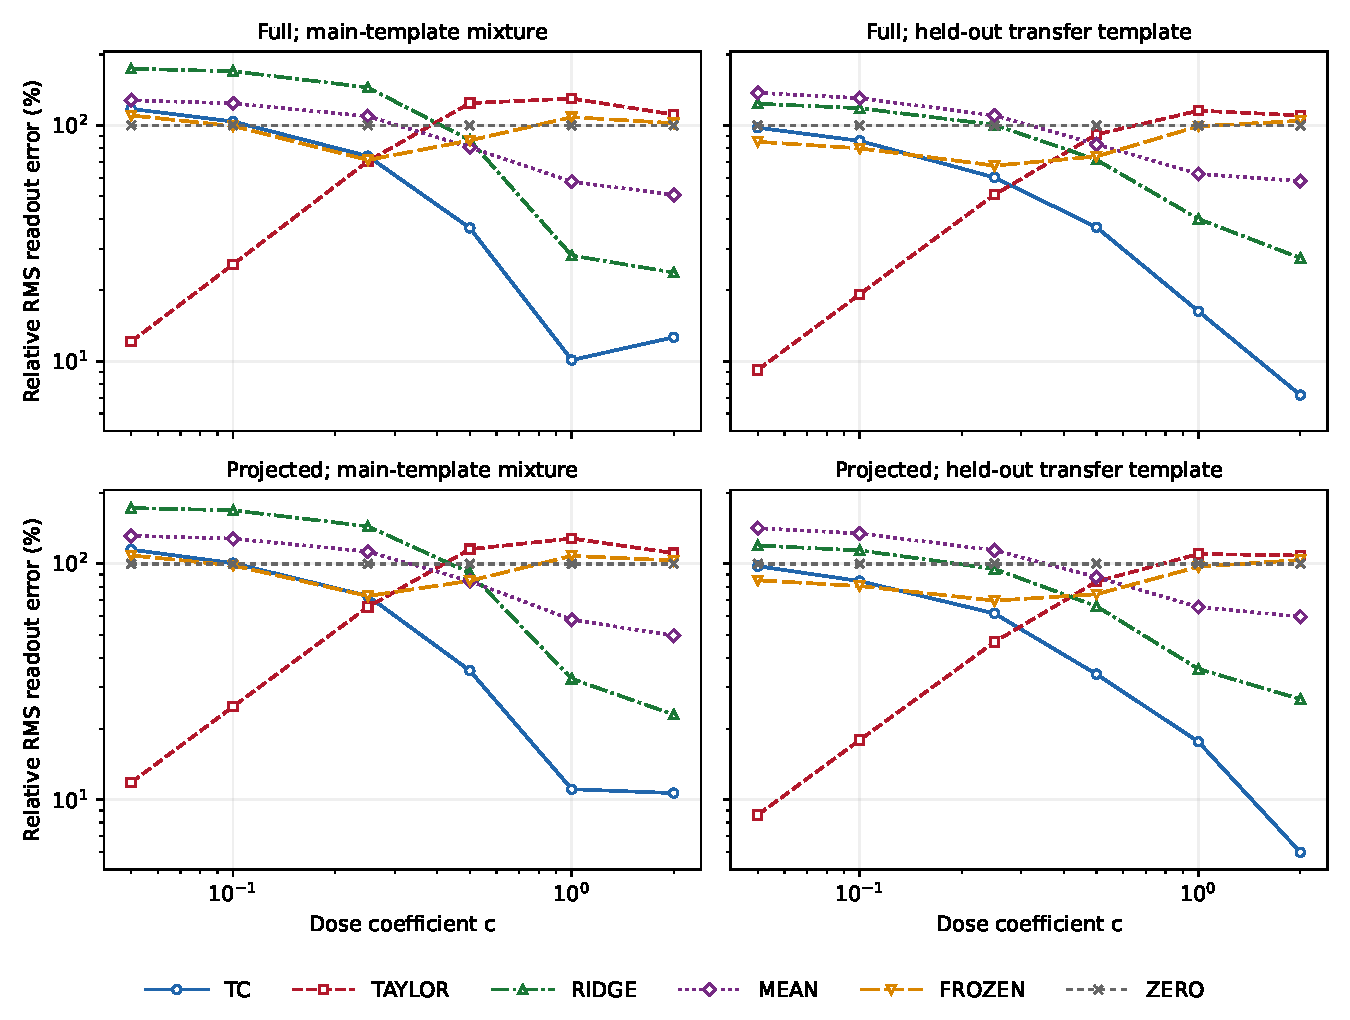
\includegraphics[width=\linewidth]{figures/new_test_dose.pdf}
\caption{All six Gemma-270M TEST doses, main mixture and transfer; pooled relative RMS error. Full numerical grids are in the supplement.}\label{fig:dose}
\end{figure}

\subsection{Gemma-1B: the crossover repeats, the accuracy does not}\label{sec:second}
The second artifact repeats Taylor's small-dose advantage and large-dose failure, but at the full patch its transcoder error, 115.38\% (nominal interval [112.72\%, 118.25\%]), exceeds zero change, ridge and the class mean (Table~\ref{tab:second}). In absolute terms it is .4406 logits against a native signal of .3819. At dose 2 it beats zero change and has a point error close to the class mean (41.86\% versus 43.73\%), but loses to ridge. A small native signal alone does not obviously explain the failure: at 270M doses with similarly small signals ($c=.25$ and $.5$), the 270M transcoder still has 74\% and 37\% error against ridge's 145\% and 87\%, although artifact, model, layer and suffix all differ, so this comparison does not isolate a cause. Crossover and useful accuracy are therefore empirically separable: a replacement can dominate a poor local approximation without predicting the intervention well.

\begin{table}[ht]\centering\small
\begin{tabular}{lrrrrr}\toprule Condition & TC & Taylor & Ridge & Mean & Zero\\\midrule
Main, $c=.05$ & 134.18 & 23.56 & 84.78 & 94.91 & 100\\
Main, $c=1$ & 115.38 & 269.86 & 50.80 & 66.99 & 100\\
Main, $c=2$ & 41.86 & 110.86 & 34.63 & 43.73 & 100\\
Transfer, $c=1$ & 137.43 & 267.26 & 60.81 & 74.98 & 100\\\bottomrule\end{tabular}
\caption{Gemma-1B relative RMS error, percent, on 256 further blocks. All 144 cells are in the supplement.}\label{tab:second}
\end{table}

\begin{figure}[ht]\centering
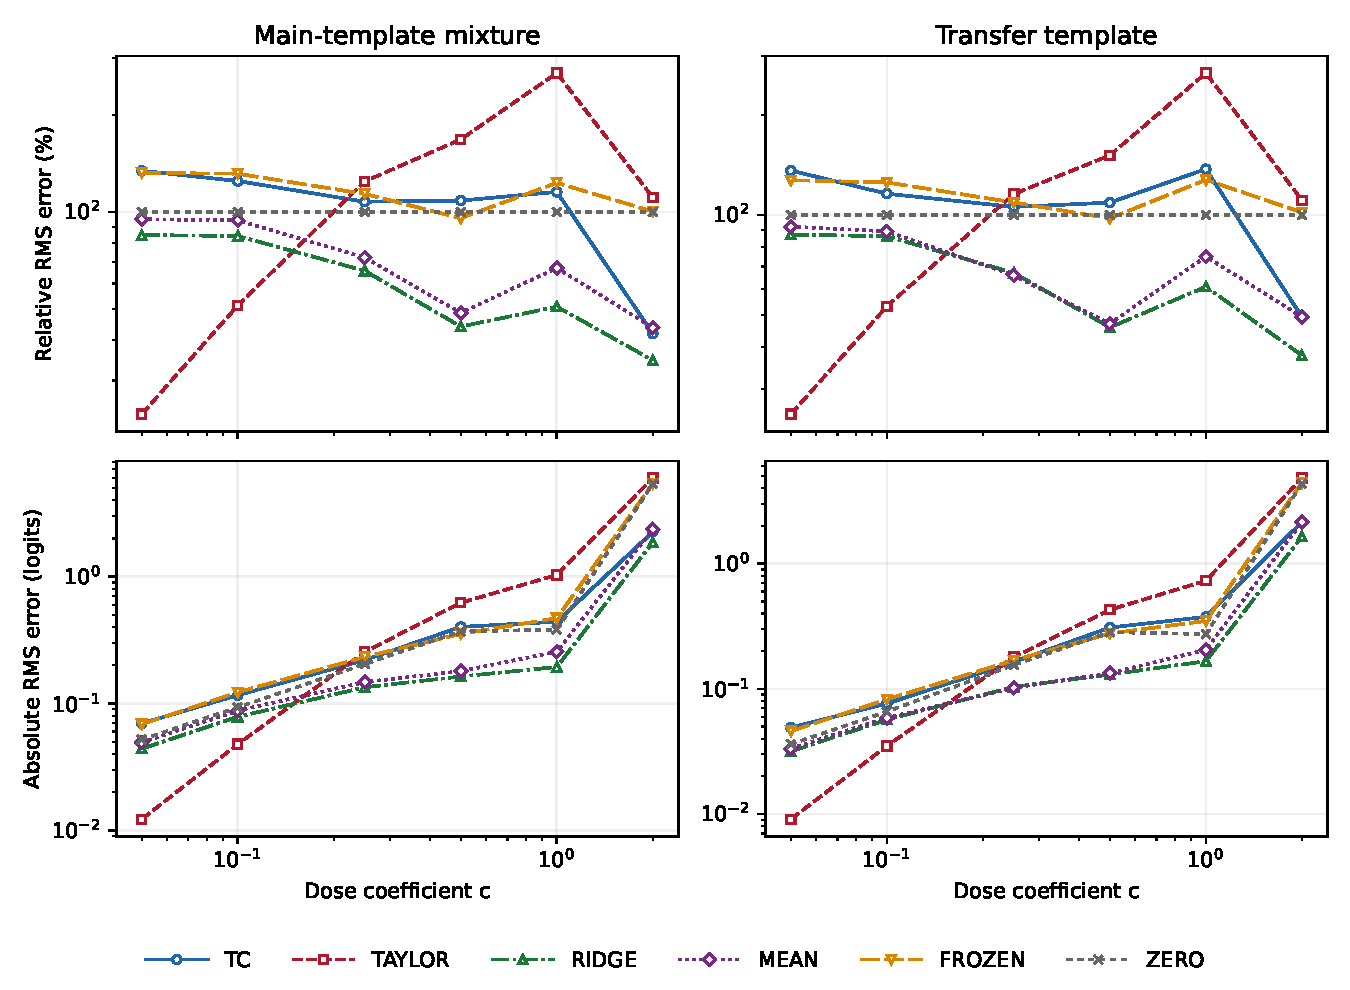
\includegraphics[width=\linewidth]{figures/second_artifact_dose.pdf}
\caption{Gemma-1B layer-22 dose curves, main mixture and transfer; top: relative RMS error, bottom: absolute RMS error (logits). Relative and absolute rankings agree within each condition.}\label{fig:second}
\end{figure}

\section{What the first artifact's error looks like}
\subsection{Endpoint cancellation}
With endpoint reconstruction errors $e_0=T(z)-f(z)$ and $e_1=T(z+\delta)-f(z+\delta)$, the predicted delta error is $e_1-e_0$, with energy $\mathbb E\|e_1\|^2+\mathbb E\|e_0\|^2-2\mathbb E(e_1^\top e_0)$. At the full patch each endpoint carries energy $1.36\times10^6$, yet the delta error carries only $.71\times10^6$: most reconstruction error is shared between endpoints and cancels. The cancelling part is a per-template mean offset; after centering within each template, the remaining cross contribution slightly increases the delta error. A shared offset cancels in any predictor evaluated as a difference, so this alone does not explain why this artifact is accurate. These statistics pool all three templates. Cancellation shrinks the vector error, but the vector residual still grows with dose (RMS 95.3 at $c=.05$ to 840.6 at $c=1$), so the readout result also depends on how the native suffix filters that residual: at $c=1$ the natural-point gradient term has RMS .267 logits against an observed readout-error RMS of .345, with a nonlinear remainder of RMS .127.

\subsection{Residual direction and threshold switches}
On 32 previously observed blocks (768 conditions), replacing each full-dose residual with a partner residual of the same norm (cyclic shifts 1 and 7) increases readout MSE from .11153 to .14940/.18659 for full edits and from .12119 to .23641/.25200 for projected edits; every full-dose frame favors the original direction. The transcoder's residual is thus oriented favorably for this readout, not merely small.

A mask decomposition shows where the large-dose response is carried. Writing the endpoint code as a base term with the baseline mask plus the contribution of features that switch, we either keep only the switches of 32 FIT-selected features (ONLY) or all switches except theirs (EXCEPT). At full dose, ONLY gives MSE .10463, essentially the original .11153, while EXCEPT gives 8.93294 (projected: .11782 and 7.45841 versus .12119). The selected group contributes on average 8.3 threshold crossings per context at full dose (4.1 for projected edits); ONLY retains the whole base code, so the result shows that these switches are necessary for accuracy rather than that they alone produce it. The fixed random 32-feature group rarely switches (no switches in 188/192 contexts) and is not a strength-matched control.

To compare directions at equal strength, we rescale each group's summed switch contribution to a fixed norm, $y_G=y_{\mathrm{TC\_FULL}}-\rho S_G/\|S_G\|$, with groups and $\rho$ fixed on FIT. Removing the top32 direction damages prediction far more than removing five alternative directions (Table~\ref{tab:norm}), on observed and on 32 fresh lexical blocks; the alternatives change the error little (slightly improving it on the observed blocks, near zero with mixed signs on the fresh ones). At equal norm the top32 direction moves the readout about fifteen times as much (mean absolute effect .297 versus about .019 on the observed blocks; .312 versus about .019 on the fresh ones), so the contrast largely reflects readout sensitivity to that direction. The alternatives overlap (one to four distinct directions per context), and top32 was selected by its contribution to the transcoder prediction, so this contrast shows that the prediction's accuracy is concentrated in those switches; it does not identify a native circuit. A control along the transcoder's own predicted delta and a gradient at TC\_FULL would separate prediction-alignment from readout sensitivity; the MSE increment decomposes exactly as $(\Delta m)^2+2e\Delta m$, so both matter.

\begin{table}[ht]\centering\small
\begin{tabular}{lrrr}\toprule Cohort/frame & Eligible contexts & Blocks & Top minus controls\\\midrule
Observed so/when & 128/128 & 32/32 & .165807\\
Fresh lexical so/when & 128/128 & 32/32 & .198352\\
Fresh changed context & 45/64 & 26/32 & .083652\\
Fresh object/readout & 12/64 & 9/32 & .013883\\\bottomrule\end{tabular}
\caption{Full-dose fixed-norm direction diagnostic, squared-logit MSE increment; positive means more damage from removing the top32 direction. Descriptive; coverage requires eligibility of all six groups.}\label{tab:norm}
\end{table}

\section{A negative boundary: a Qwen CLT component}
The public Qwen3-0.6B-Base cross-layer transcoder component from source layer 27 to target layer 27, under an input edit at layer 27 (earlier-source contributions stay fixed and cancel, so this tests the single source-27 component, not the whole CLT), evaluated through the final norm and head for is/are on 256 blocks shared with the companion study, stays at the zero-change baseline at every dose, as does its frozen-mask variant (Table~\ref{tab:qwen}): at full dose its absolute error is 2.455 logits against a native signal of 2.447, while Taylor has .847 and ridge .748. The operator passed hook, head, JVP and reachability checks. A favorable regime is thus not a generic property of public replacement components; model, layer, readout and artifact type all differ, so the contrast does not isolate a cause.

\begin{table}[ht]\centering\small
\begin{tabular}{lrr}\toprule Predictor & $c=.05$ & $c=1$\\\midrule
CLT component & 99.830 & 100.347\\
Native-vector Taylor & 3.172 & 34.600\\
Composed scalar linear & 3.305 & 35.904\\
Frozen recipient mask & 99.830 & 100.302\\
FIT ridge & 36.499 & 30.572\\
FIT conditional mean & 37.589 & 37.757\\
Zero change & 100.000 & 100.000\\\bottomrule\end{tabular}
\caption{Qwen component relative RMS error, percent, T2/T5 mixture.}\label{tab:qwen}
\end{table}

\section{Discussion}
Local fidelity, ranking against local linearization and finite-effect accuracy are three different properties of a replacement model. The two Gemma artifacts tested under the frozen protocol separate them in different ways, whereas the Qwen component is poor on all three. The Gemma-270M transcoder is a poor local model yet predicts full-patch effects to about 10\%, better in readout than a ridge map that is closer in vector space; the Gemma-1B transcoder shows the same crossover without that accuracy; the Qwen CLT component shows neither. For anyone using a transcoder to predict or choose interventions, the practical consequence is that fidelity should be measured at the intervention size of interest, in the readout of interest and against learned and zero-change baselines, rather than inferred from reconstruction, Jacobians or superiority to Taylor.

The scope is one historically selected public artifact with a clear positive result, one replication of the crossover, synthetic pronoun contexts and two-token readouts; the original hypothesis family was not qualified, and the mechanism diagnostics are posthoc. Within that scope the first artifact's success is associated with a favorably oriented residual and the threshold switches of one FIT-selected group, while endpoint-error cancellation alone does not explain it; a predictive account of which artifacts reach this regime remains open. Complete dose grids, earlier hypotheses and failed forecasts, operation accounting and independent reviews are in the supplement. Complete per-template dose grids and the second-artifact curves are given in the appendix; the full historical record, operation accounting and independent reviews are available with the evidence bundle.

\paragraph{Use of AI tools.} AI assistants were used for code development, analysis support, literature search and editing of the text. All experimental designs, results and claims were checked by the author, who takes full responsibility for the content.

\paragraph{Code and data availability.} Code, frozen protocols, per-condition results, summary files and the full supplementary record are available at \url{https://github.com/rafalwronapl/interp-transcoder-dose}.

\clearpage
{\small
\bibliographystyle{plain}
\bibliography{references}}
\appendix
\section{Protocol summary}\label{app:protocol}
\textbf{Gemma-270M.} Public medium Gemma Scope~2 transcoder for layer 15 (16k features, JumpReLU, no affine skip); boundary at the post-feedforward-normalized branch output, final token. FIT: 32 name-pair blocks (128 natural states, so/when) fix the class-mean direction $w$, class-cell means and per-cell ridge maps ($\lambda=.01$, centered intercept, global input RMS). PILOT: 32 further blocks. TEST: 256 disjoint blocks $\times$ two sides $\times$ three templates (1,536 recipients), six doses, full and projected operators, 18,432 scored cells. Every prediction is inserted into the native branch output and propagated through native layers 16--17 (dynamic attention), final norm and head; readout is the she-minus-he logit margin. FP32 throughout, with qualified exact-prefix/suffix parity. Intervals: 99\% paired studentized log-RMS max-statistic intervals for the 12 full-dose transcoder metrics, qualified on eight synthetic scenarios before TEST; 11/12 width targets met.

\textbf{Gemma-1B.} Public medium 16k layer-22 transcoder ($L_0=60$, no affine skip); 32 fresh FIT and 256 fresh TEST blocks; full operator, six doses; suffix layers 23--25 and head; nominal 95\% block-bootstrap intervals (1,999 draws).

\textbf{Qwen3-0.6B.} Public BlueLightAI 20k cross-layer transcoder, source-27 to target-27 component; input edit on the normalized MLP input; six doses; final RMSNorm and is-minus-are head readout; 256 blocks, two frames, 2,048 contexts.

\textbf{Diagnostics.} Residual substitutions and mask arms use 32 previously observed 270M TEST blocks (768 conditions); the fixed-norm direction study uses cached FIT (32 blocks), the same 32 observed blocks and 32 fresh lexical blocks. All diagnostic outputs are scored through the exact native suffix.

\section{Complete new TEST grid}\label{app:fullgrid}
All entries below are relative RMS readout errors in percent. Each cell uses all 256 blocks. No intervals or population decisions are assigned to this full grid.
\subsection{Full: so}
\begin{center}\small\begin{tabular}{lrrrrrr}
\toprule Method & .05 & .1 & .25 & .5 & 1 & 2\\
\midrule
TC & 113.64 & 100.20 & 74.75 & 32.79 & 9.58 & 14.67\\
TAYLOR & 11.40 & 24.16 & 66.60 & 121.01 & 128.21 & 108.79\\
FROZEN & 109.93 & 97.93 & 70.17 & 89.65 & 109.10 & 98.77\\
MEAN & 124.39 & 121.06 & 107.54 & 79.80 & 55.64 & 49.31\\
RIDGE & 175.99 & 171.11 & 146.18 & 89.68 & 28.18 & 21.93\\
ZERO & 100.00 & 100.00 & 100.00 & 100.00 & 100.00 & 100.00\\
\bottomrule\end{tabular}\end{center}
\subsection{Full: when}
\begin{center}\small\begin{tabular}{lrrrrrr}
\toprule Method & .05 & .1 & .25 & .5 & 1 & 2\\
\midrule
TC & 124.24 & 110.51 & 72.51 & 43.43 & 11.01 & 8.39\\
TAYLOR & 13.30 & 28.58 & 78.03 & 130.42 & 133.05 & 114.77\\
FROZEN & 110.58 & 102.12 & 73.63 & 79.37 & 106.98 & 107.46\\
MEAN & 133.67 & 129.55 & 112.92 & 82.57 & 61.30 & 52.82\\
RIDGE & 169.70 & 166.57 & 141.57 & 80.25 & 27.82 & 26.42\\
ZERO & 100.00 & 100.00 & 100.00 & 100.00 & 100.00 & 100.00\\
\bottomrule\end{tabular}\end{center}
\subsection{Full: transfer}
\begin{center}\small\begin{tabular}{lrrrrrr}
\toprule Method & .05 & .1 & .25 & .5 & 1 & 2\\
\midrule
TC & 97.78 & 85.94 & 60.13 & 36.99 & 16.28 & 7.19\\
TAYLOR & 9.18 & 19.21 & 50.84 & 91.49 & 115.44 & 110.20\\
FROZEN & 85.19 & 79.92 & 67.51 & 73.81 & 99.15 & 104.59\\
MEAN & 137.39 & 130.41 & 110.19 & 83.22 & 62.23 & 58.02\\
RIDGE & 123.59 & 118.25 & 100.49 & 71.48 & 40.10 & 27.36\\
ZERO & 100.00 & 100.00 & 100.00 & 100.00 & 100.00 & 100.00\\
\bottomrule\end{tabular}\end{center}
\subsection{Full: so/when pooled (main mixture)}
\begin{center}\small\begin{tabular}{lrrrrrr}
\toprule Method & .05 & .1 & .25 & .5 & 1 & 2\\
\midrule
TC & 117.46 & 103.77 & 74.04 & 36.73 & 10.11 & 12.63\\
TAYLOR & 12.10 & 25.72 & 70.44 & 124.27 & 129.96 & 111.13\\
FROZEN & 110.16 & 99.35 & 71.29 & 86.32 & 108.35 & 102.20\\
MEAN & 127.72 & 123.97 & 109.28 & 80.75 & 57.73 & 50.69\\
RIDGE & 173.81 & 169.60 & 144.73 & 86.61 & 28.05 & 23.76\\
ZERO & 100.00 & 100.00 & 100.00 & 100.00 & 100.00 & 100.00\\
\bottomrule\end{tabular}\end{center}
\subsection{Projected: so}
\begin{center}\small\begin{tabular}{lrrrrrr}
\toprule Method & .05 & .1 & .25 & .5 & 1 & 2\\
\midrule
TC & 107.74 & 95.46 & 72.06 & 29.74 & 10.62 & 12.27\\
TAYLOR & 11.66 & 24.32 & 62.60 & 108.86 & 123.43 & 107.76\\
FROZEN & 105.10 & 94.83 & 71.59 & 86.84 & 107.51 & 99.57\\
MEAN & 128.96 & 125.40 & 109.17 & 81.62 & 56.62 & 48.51\\
RIDGE & 178.84 & 174.08 & 145.77 & 91.79 & 32.29 & 21.87\\
ZERO & 100.00 & 100.00 & 100.00 & 100.00 & 100.00 & 100.00\\
\bottomrule\end{tabular}\end{center}
\subsection{Projected: when}
\begin{center}\small\begin{tabular}{lrrrrrr}
\toprule Method & .05 & .1 & .25 & .5 & 1 & 2\\
\midrule
TC & 127.35 & 110.08 & 75.33 & 46.04 & 11.90 & 7.71\\
TAYLOR & 12.07 & 25.74 & 71.93 & 129.95 & 136.76 & 115.52\\
FROZEN & 114.93 & 105.16 & 76.19 & 79.18 & 109.13 & 108.46\\
MEAN & 136.11 & 132.56 & 120.20 & 91.15 & 60.43 & 51.11\\
RIDGE & 159.37 & 156.94 & 140.48 & 91.33 & 32.99 & 24.39\\
ZERO & 100.00 & 100.00 & 100.00 & 100.00 & 100.00 & 100.00\\
\bottomrule\end{tabular}\end{center}
\subsection{Projected: transfer}
\begin{center}\small\begin{tabular}{lrrrrrr}
\toprule Method & .05 & .1 & .25 & .5 & 1 & 2\\
\midrule
TC & 97.73 & 84.48 & 61.58 & 34.04 & 17.59 & 5.98\\
TAYLOR & 8.61 & 17.90 & 46.62 & 84.03 & 110.05 & 108.46\\
FROZEN & 85.13 & 80.49 & 69.79 & 74.30 & 97.19 & 103.83\\
MEAN & 141.60 & 134.42 & 114.09 & 87.82 & 65.58 & 59.63\\
RIDGE & 119.62 & 113.91 & 95.13 & 66.09 & 35.83 & 26.66\\
ZERO & 100.00 & 100.00 & 100.00 & 100.00 & 100.00 & 100.00\\
\bottomrule\end{tabular}\end{center}
\subsection{Projected: so/when pooled (main mixture)}
\begin{center}\small\begin{tabular}{lrrrrrr}
\toprule Method & .05 & .1 & .25 & .5 & 1 & 2\\
\midrule
TC & 114.83 & 100.60 & 73.07 & 35.25 & 11.07 & 10.66\\
TAYLOR & 11.80 & 24.81 & 65.58 & 115.36 & 128.09 & 110.98\\
FROZEN & 108.57 & 98.42 & 73.02 & 84.69 & 108.06 & 103.27\\
MEAN & 131.45 & 127.85 & 112.64 & 84.49 & 57.94 & 49.59\\
RIDGE & 172.42 & 168.52 & 144.18 & 91.65 & 32.53 & 22.92\\
ZERO & 100.00 & 100.00 & 100.00 & 100.00 & 100.00 & 100.00\\
\bottomrule\end{tabular}\end{center}

\section{Complete second-artifact dose curves}\label{app:secondcurve}
All 144 accepted metric cells are represented below. Entries are relative RMS error in percent; zero change is 100\%. The four aggregations share lexical blocks and are not independent replications. Absolute errors, native signal RMS and nominal pointwise intervals remain in the copied \texttt{summary.json}.
\begin{table}[!ht]\centering\small
\begin{tabular}{rrrrrrr}\toprule
$c$ & TC & Taylor & Ridge & Mean & Frozen & Zero\\\midrule
0.05 & 144.950 & 20.334 & 86.001 & 95.105 & 140.885 & 100.000\\
0.1 & 134.078 & 45.995 & 87.640 & 96.190 & 140.393 & 100.000\\
0.25 & 104.719 & 129.339 & 75.441 & 79.659 & 117.446 & 100.000\\
0.5 & 102.126 & 182.199 & 49.052 & 51.870 & 85.382 & 100.000\\
1 & 99.014 & 277.650 & 57.057 & 71.287 & 125.349 & 100.000\\
2 & 44.607 & 112.115 & 36.066 & 45.731 & 100.060 & 100.000\\
\bottomrule\end{tabular}
\caption{Gemma-3-1B L22, full donor edits; so. All six frozen doses and all methods, 256 TEST blocks.}\end{table}
\begin{table}[!ht]\centering\small
\begin{tabular}{rrrrrrr}\toprule
$c$ & TC & Taylor & Ridge & Mean & Frozen & Zero\\\midrule
0.05 & 113.331 & 28.251 & 82.652 & 94.586 & 115.693 & 100.000\\
0.1 & 108.760 & 58.410 & 78.559 & 90.944 & 116.275 & 100.000\\
0.25 & 110.292 & 119.271 & 54.324 & 63.859 & 109.902 & 100.000\\
0.5 & 114.420 & 152.639 & 38.505 & 45.129 & 104.836 & 100.000\\
1 & 134.084 & 259.131 & 41.017 & 60.818 & 120.098 & 100.000\\
2 & 38.657 & 109.476 & 32.992 & 41.452 & 100.580 & 100.000\\
\bottomrule\end{tabular}
\caption{Gemma-3-1B L22, full donor edits; when. All six frozen doses and all methods, 256 TEST blocks.}\end{table}
\begin{table}[!ht]\centering\small
\begin{tabular}{rrrrrrr}\toprule
$c$ & TC & Taylor & Ridge & Mean & Frozen & Zero\\\midrule
0.05 & 136.021 & 25.155 & 87.313 & 92.249 & 127.200 & 100.000\\
0.1 & 115.874 & 53.109 & 86.261 & 89.201 & 125.302 & 100.000\\
0.25 & 105.742 & 115.604 & 66.921 & 65.792 & 109.029 & 100.000\\
0.5 & 108.948 & 151.164 & 45.891 & 47.094 & 97.704 & 100.000\\
1 & 137.426 & 267.259 & 60.812 & 74.980 & 127.552 & 100.000\\
2 & 49.322 & 110.761 & 37.800 & 49.351 & 101.766 & 100.000\\
\bottomrule\end{tabular}
\caption{Gemma-3-1B L22, full donor edits; transfer. All six frozen doses and all methods, 256 TEST blocks.}\end{table}
\begin{table}[!ht]\centering\small
\begin{tabular}{rrrrrrr}\toprule
$c$ & TC & Taylor & Ridge & Mean & Frozen & Zero\\\midrule
0.05 & 134.182 & 23.559 & 84.784 & 94.915 & 132.173 & 100.000\\
0.1 & 124.742 & 51.235 & 84.188 & 94.163 & 131.443 & 100.000\\
0.25 & 107.569 & 124.358 & 65.634 & 72.116 & 113.700 & 100.000\\
0.5 & 108.469 & 168.018 & 44.077 & 48.605 & 95.639 & 100.000\\
1 & 115.381 & 269.857 & 50.797 & 66.994 & 123.122 & 100.000\\
2 & 41.862 & 110.859 & 34.627 & 43.733 & 100.309 & 100.000\\
\bottomrule\end{tabular}
\caption{Gemma-3-1B L22, full donor edits; main\_mixture. All six frozen doses and all methods, 256 TEST blocks.}\end{table}


\end{document}
